\lecture{6}{10. September 2025}{Differential Analysis II: Kinematics \& Navier-Stokes Equations}

\subsection{Motion of a Fluid Particle (Kinematics)}
On \Cref{fig:f5_4} a typical finite fluid element is shown. Within this an infinitesimal particle with mass $\mathrm{d}m$ and initial volume $\mathrm{d}x \, \mathrm{d}y \, \mathrm{d}z$, at time $t$ as well as how it may look after an infinitesimal time interval $\mathrm{d}t$. After this period the finite element has moved and changed its shape. We will examine the infinitesimal particle so that we eventually obtain results applicable to a point. We wan decompose this infinitesimal particle's motion into four components:
\begin{itemize}
  \item translation, where the particle moves from one point to another
  \item rotation, which can occur about any or all of the $x$, $y$ or $z$ axes
  \item liner deformation, in which the particle's sides stretch or contract
  \item angular deformation, in which angles that were initially \ang{90} between the sides of the particle changes
\end{itemize}

\begin{figure} [ht]
  \centering
  
\includegraphics[width=0.8\linewidth]{./figures/f5_4.png}
  \caption{Finite fluid element and infinitesimal particle at times $t$ and $t + \mathrm{d}t$}
  \label{fig:f5_4}
\end{figure}

\begin{figure} [ht]
  \centering
  
\includegraphics[width=0.8\linewidth]{./figures/f5_5.png}
  \caption{Pictorial representation of the components of fluid motion.}
\end{figure}

\subsubsection{Fluid Translation: Acceleration of a Fluid Particle in a Velocity Field}
We will need the acceleration of a fluid particle to be able to apply Newton's second law to it. 

Consider a particle moving in a velocity field. At time, $t$, the particle is in position $x,y, z$ and has a velocity vector corresponding to the velocity at that point in space at time $t$,
\[ 
\textbf{V}_P \bigg)_t = \textbf{V}(x,y,z,t)
.\]
At time $t + \mathrm{d}t$ the particle has moved to a new position with coordinates $x + \mathrm{d}x, y + \mathrm{d}y, z + \mathrm{d}z$ and its velocity will when be given by
\[ 
\textbf{V}_P \bigg)_{t + \mathrm{d}t} = \textbf{V} \left( x + \mathrm{d}x, y + \mathrm{d}y, z + \mathrm{d}z, t + \mathrm{d}t \right)
.\]

If the particle velocity at time $t$ (position $\textbf{r}$) is given by $\textbf{V}_P = \textbf{V}(x,y,z,t)$, then $\mathrm{d}\textbf{V}_p$ is given by the chain rule as:
\[ 
\mathrm{d}\textbf{V}_p = \frac{\partial \textbf{V}}{\partial x} \, \mathrm{d}x_p + \frac{\partial \textbf{V}}{\partial y} \, \mathrm{d}y_p + \frac{\partial \textbf{V}}{\partial z} \, \mathrm{d}z_p + \frac{\partial \textbf{V}}{\partial t}\, \mathrm{d}t 
.\]
The total acceleration of the particle is given by:
\[ 
\textbf{a}_p = \frac{\mathrm{d}\textbf{V}_p}{\mathrm{d}t} = \frac{\partial \textbf{V}}{\partial x} \frac{\mathrm{d}x_p}{\mathrm{d}t} + \frac{\partial \textbf{V}}{\partial y} \frac{\mathrm{d}y_p}{\mathrm{d}t} + \frac{\partial \textbf{V}}{\partial z} \frac{\mathrm{d}z_p}{\mathrm{d}t} + \frac{\partial \textbf{V}}{\partial t}
.\]
And since
\[ 
\frac{\mathrm{d}x_p}{\mathrm{d}t} = u, \quad \frac{\mathrm{d}y_p}{\mathrm{d}t} = v, \quad \frac{\mathrm{d}z_p}{\mathrm{d}t} = w
\]
we have
\[ 
  \textbf{a}_p = \frac{\mathrm{d}\textbf{V}_p}{\mathrm{d}t} = u \frac{\partial \textbf{V}}{\partial x} + v \frac{\partial \textbf{V}}{\partial y} + w \frac{\partial \textbf{V}}{\partial z} + \frac{\partial \textbf{V}}{\partial t} 
.\]

A special symbol $\frac{\mathrm{D}\textbf{V}}{\mathrm{D}t}$ is given to the derivative to remind us that it is not simply a normal derivative, thus:
\[ 
\frac{\mathrm{D}\textbf{V}}{\mathrm{D}t} \equiv \textbf{a}_p = u \frac{\partial \textbf{V}}{\partial x} + v \frac{\partial \textbf{V}}{\partial y} + w \frac{\partial \textbf{V}}{\partial z} + \frac{\partial \textbf{V}}{\partial t}
.\]
This derivative is sometimes called the \textit{substantial derivative}, the \textit{material derivative} or the \textit{particle derivative}. 

From this we see that a fluid particle moving in a flow field may accelerate for either of two reasons. Either through \textit{convective acceleration}, where fluid particles are \textit{convected} between regions with different velocities. If the flow field is unsteady an additional \textit{local acceleration} is applied, because the velocity field is then a function of time.

The convective acceleration can be written using the gradient operator as:
\[ 
u \frac{\partial \textbf{V}}{\partial x} + v \frac{\partial \textbf{V}}{\partial y} + w \frac{\partial \textbf{V}}{\partial z} = \left( \textbf{V} \cdot \nabla  \right) \textbf{V}
.\]
Thus the acceleration may be written as:
\[ 
\frac{\mathrm{D}\textbf{V}}{\mathrm{D}t} \equiv \textbf{a}_p = \left( \textbf{V} \cdot \nabla  \right)\textbf{V} + \frac{\partial \textbf{V}}{\partial t}
.\]
For a two dimensional flow, this becomes:
\[ 
\frac{\mathrm{D}\textbf{V}}{\mathrm{D}t} = u \frac{\partial \textbf{V}}{\partial x} + v \frac{\partial \textbf{V}}{\partial y} + \frac{\partial \textbf{V}}{\partial t}
.\]
For a one dimensional flow it becomes:
\[ 
  \frac{\mathrm{D}\textbf{V}}{\mathrm{D}t} = u \frac{\partial \textbf{V}}{\partial x} + \frac{\partial \textbf{V}}{\partial t} 
.\]
And finally for a steady flow in three dimensions it becomes:
\[ 
\frac{\mathrm{D}\textbf{V}}{\mathrm{D}t} = u \frac{\partial \textbf{V}}{\partial x} + v \frac{\partial \textbf{V}}{\partial y} + w \frac{\partial \textbf{V}}{\partial z}
.\]
This means that a fluid particle may undergo convective acceleration even in a steady velocity field simply due to its motion. As scalar component equation we have
\begin{align*}
  a_{x_p} &= \frac{\mathrm{D}u}{\mathrm{D}t} = u \frac{\partial u}{\partial x} + v \frac{\partial u}{\partial y} + w \frac{\partial u}{\partial z} + \frac{\partial u}{\partial t} \\
    a_{y_p} &= \frac{\mathrm{D}v}{\mathrm{D}t} = u \frac{\partial v}{\partial x} + v \frac{\partial v}{\partial y} + w \frac{\partial v}{\partial z} + \frac{\partial v}{\partial t} \\
  a_{z_p} &= \frac{\mathrm{D}w}{\mathrm{D}t} = u \frac{\partial w}{\partial x} + v \frac{\partial w}{\partial y} + w \frac{\partial w}{\partial z} + \frac{\partial w}{\partial t}
.\end{align*}


\subsubsection{Fluid Rotation} \label{sec:rot}
The fluid particle may rotate about all coordinate axes. In general,
\[ 
  \boldsymbol{\omega} = \hat{i} \omega_x + \hat{j} \omega_y + \hat{k} \omega_z
.\]

We now consider the $xy$ plane view of the particle at time $t$ on \Cref{fig:f5_7}. The left and lower sides of the particle are given by the two perpendicular line segments $oa$ and $ob$ of length $\Delta x$ and $\Delta y$, respectively. After a time interval $\Delta t$ the particle will have translated to some new position and also have rotated and deformed.

These two sides may now have deformed by the same angle $\Delta \alpha$ and $\Delta \beta$. To extract a rotation from this one takes the average of the rotations of $\Delta \alpha$ and $\Delta \beta$ such that the counterclockwise rotation is $\frac{1}{2} \left( \Delta \alpha - \Delta \beta \right)$. 

\begin{figure} [ht]
  \begin{subfigure}{0.24\linewidth}
    \centering
    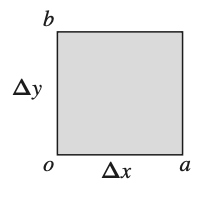
\includegraphics[width=\linewidth]{./figures/f5_7a.png}
    \caption{Original particle}
  \end{subfigure}
  \begin{subfigure}{0.24\linewidth}
    \centering
    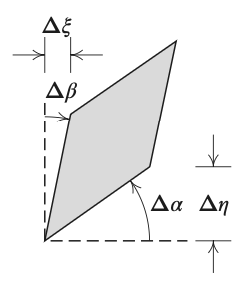
\includegraphics[width=\linewidth]{./figures/f5_7b.png}
    \caption{Particle after time $\Delta t$}
  \end{subfigure}
  \begin{subfigure}{0.24\linewidth}
    \centering
    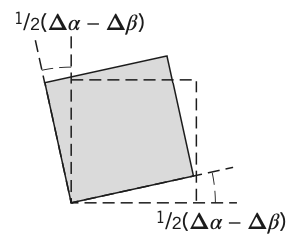
\includegraphics[width=\linewidth]{./figures/f5_7c.png}
    \caption{Rotational component}
  \end{subfigure}
  \begin{subfigure}{0.24\linewidth}
    \centering
    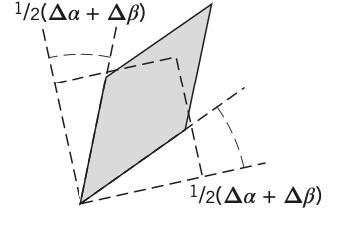
\includegraphics[width=\linewidth]{./figures/f5_7d.png}
    \caption{Angular deformation component}
  \end{subfigure}
  \caption{Rotation and angular deformation of perpendicular line segments in a two-dimensional flow.}
  \label{fig:f5_7}
\end{figure}

From $\Delta \alpha$ and $\Delta \beta$ we can also determine a measure of the particle's angular deformation. To obtain the deformation of side $oa$ we subtract the particle rotation $\frac{1}{2}\left( \Delta \alpha - \Delta \beta \right)$ from the actual rotation of $oa$, $\Delta \alpha$, what remains is the deformation of side $oa$. The total deformation of the particle is the sum of the deformations of the sides or $\Delta \alpha + \Delta \beta$. 

Now we need to convert these angular measures to quantities obtainable from the flow field. To do this, we recognize that for small angles $\Delta \alpha = \frac{\Delta \eta}{\Delta x}$, and $\Delta \beta = \frac{\Delta\xi}{\Delta y}$. $\Delta \xi$ arises because, if in an interval $\Delta t$ point $o$ moves horizontally distance $u \Delta t$ then point $b$ will have moved a distance $\left( u + \left( \frac{\partial u}{\partial y} \right)\Delta y \right)\Delta t$. Likewise for $\Delta \eta$. Hence,
\begin{align*}
  \Delta \xi &=  \left( u + \frac{\partial u}{\partial y} \Delta y \right) \Delta t - u \Delta t = \frac{\partial u}{\partial y} \Delta y \Delta t \\
  \Delta \eta &= \left( v + \frac{\partial v}{\partial x}\Delta x \right) \Delta t - v \Delta t = \frac{\partial v}{\partial x} \Delta x \Delta t
.\end{align*}
We can now compute the angular velocity of the particle about the $z$ axis $\omega_z$ by combining all these results:
\begin{align*}
  \omega_z &= \lim_{\Delta t \to 0} \frac{\frac{1}{2} \left( \Delta \alpha - \Delta \beta \right)}{\Delta t} \\
  &= \lim_{\Delta t \to 0} \frac{\frac{1}{2} \left( \frac{\Delta \eta}{\Delta x} - \frac{\Delta \xi}{\Delta y}\right)}{\Delta t} \\
  &= \lim_{\Delta t \to 0} \frac{\frac{1}{2} \left( \frac{\partial v}{\partial x} \frac{\Delta x}{\Delta x} \Delta t - \frac{\partial u}{\partial y} \frac{\Delta y}{\Delta y} \Delta t \right)}{\Delta t} \\
  &= \frac{1}{2} \left( \frac{\partial v}{\partial x} - \frac{\partial u}{\partial y}  \right)
.\end{align*}
Similarly one can show that:
\begin{align*}
  \omega_x &= \frac{1}{2} \left( \frac{\partial w}{\partial y} - \frac{\partial v}{\partial z}  \right) \\
  \omega_y &= \frac{1}{2} \left( \frac{\partial u}{\partial z} - \frac{\partial w}{\partial x}  \right)
.\end{align*}
Then $\boldsymbol{\omega}$ becomes:
\[ 
  \boldsymbol{\omega} = \frac{1}{2} \left( \hat{i} \left( \frac{\partial w}{\partial y} - \frac{\partial v}{\partial z}  \right) + \hat{j} \left( \frac{\partial u}{\partial z} - \frac{\partial w}{\partial x}  \right) + \hat{k} \left( \frac{\partial v}{\partial x} - \frac{\partial u}{\partial y}  \right) \right)
.\]
The term in the outermost parenthesis can be written
\[ 
  \mathrm{curl} \textbf{V} = \nabla \times \textbf{V}
.\]
And therefore we get:
\[ 
  \boldsymbol{\omega} = \frac{1}{2} \nabla  \times \textbf{V}
.\]

Fluid rotation can arise in a number of different ways. One way, if the particles are not rotating initially, for rotation to be induced is due to torque caused by surface shear stresses -- the particle body force and pressure forces cannot generate torque. Hence rotation of fluid particles will always occur when we have shear stresses.

Flows without particle rotation are called \textit{irrotational flows}. Although no real flow is truly irrotational as all fluids are viscous, many flows can be studied assuming they are inviscid and irrotational. 

The factor of $\frac{1}{2}$ can be eliminated in the expression for $\boldsymbol{\omega}$ by defining the vorticity $\boldsymbol{\xi}$ to be twice the rotation,
\[ 
  \boldsymbol{\xi} \equiv 2 \boldsymbol{\omega} = \nabla \times \textbf{V}
.\]

The \textit{circulation}, $\Gamma$, is defined as the line integral of the tangential velocity component about any closed curve fixed in the flow,
\[ 
\Gamma = \oint_c \textbf{V} \cdot \mathrm{d}\textbf{s}
\]
where $\mathrm{d}\textbf{s}$ is an elemental vector tangent to the curve with length $\mathrm{d}s$ of the element of arc. We can develop a relationship between circulation and vorticity by considering the rectangular circuit shown in \Cref{fig:f5_8}, where the velocity components at $o$ are set to $(u, v)$ and the velocities along segments $bc$ and $ac$ can be derived using Taylor series approximations.

\begin{figure} [ht]
  \centering
  
\includegraphics[width=0.65\linewidth]{./figures/f5_8.png}
  \caption{Velocity components on the boundaries of a fluid element.}
  \label{fig:f5_8}
\end{figure}

For the closed curve $oac b$ we get
\begin{align*}
  \Delta \Gamma &= u \Delta x + \left( v + \frac{\partial v}{\partial x} \Delta x \right) \Delta y - \left( u + \frac{\partial u}{\partial y} \Delta y \right) \Delta x - v \Delta y \\
  &= \left( \frac{\partial v}{\partial x} - \frac{\partial u}{\partial y}  \right) \Delta x \Delta y \\
  &= 2 \omega_z \Delta x \Delta y
.\end{align*}
Then
\begin{equation}\label{eq:stoke2d}
 \Gamma = \oint_c \textbf{V} \cdot \mathrm{d}\textbf{s} = \int_A 2 \omega_z \, \mathrm{d}A = \int_A \left( \nabla  \times \textbf{V} \right)_z \, \mathrm{d}A 
\end{equation}
\Cref{eq:stoke2d} is a statement of the Stokes theorem in two dimensions; the circulation around a closed contour is equal to the total vorticity enclosed within it. 

\subsubsection{Fluid Deformation}

\paragraph{Angular Deformation}
The total angular deformation of a particle is given by the sum of the two angular deformations, i.e. $\Delta \alpha + \Delta \beta$. We have also found $\Delta \alpha = \frac{\Delta \eta}{\Delta x}$, $\Delta \beta = \frac{\Delta \xi}{\Delta y}$ where $\Delta \xi$  and $\Delta \eta$ are given by
\begin{align*}
  \Delta \xi &= \left( u + \frac{\partial u}{\partial y} \Delta y \right)\Delta t - u \Delta t = \frac{\partial u}{\partial y} \Delta y\Delta t \\
  \Delta \eta &= \left( v + \frac{\partial v}{\partial x} \Delta x \right) \Delta t - v \Delta t = \frac{\partial v}{\partial x} \Delta x \Delta t
.\end{align*}
By combining these results we can compute the rate of angular deformation of the particle in the $xy$ as
\begin{align*}
  \text{Rate of angular deformation}_{xy} &= \lim_{\Delta t \to 0} \frac{\left( \Delta \alpha + \Delta \beta \right)}{\Delta t} \\
  &= \lim_{\Delta t \to 0} \frac{\frac{\Delta \eta}{\Delta x} + \frac{\Delta \xi}{\Delta y}}{\Delta t} \\
  &= \lim_{\Delta t \to 0} \frac{\frac{\partial v}{\partial x} \frac{\Delta x}{\Delta x} \Delta t + \frac{\partial u}{\partial y} \frac{\Delta y}{\Delta y} \Delta t}{\Delta t} \\
  &= \frac{\partial v}{\partial x} + \frac{\partial u}{\partial y}
.\end{align*}
Similar expressions can be found for the angular deformation in the $yz$ and $zx$ planes:
\begin{align*}
  \text{Rate of angular deformation}_{yz} &= \frac{\partial w}{\partial y} + \frac{\partial v}{\partial z} \\
  \text{Rate of angular deformation}_{zx} &= \frac{\partial w}{\partial x} + \frac{\partial u}{\partial z} 
.\end{align*}

We have previously shown that for one-dimensional laminar Newtonian flow the shear stress is given by the rate of deformation of the particle:
\[ 
\tau_{yx} = \mu \frac{\mathrm{d}u}{\mathrm{d}y} 
.\]
This is a special case of the expression derived above. 


\paragraph{Linear Deformation}
During linear deformation, the shape of the fluid element, described by the angles at its vertices, is unchanged. The element will change length in the $x$ direction only of $\frac{\partial u}{\partial x} \neq 0$, similarly a change in the $y$ and $z$ directions only happens for $\frac{\partial v}{\partial y} \neq 0$ and $\frac{\partial w}{\partial z} \neq 0$ respectively. 

The rate of local instantaneous \textit{volume dilation} is
\[ 
\text{Volume dilation rate} = \frac{\partial u}{\partial x} + \frac{\partial v}{\partial y} + \frac{\partial w}{\partial z}  = \nabla \cdot \textbf{V}
.\]
For incompressible flow, the rate of volume dilation is zero. 


\subsection{Momentum Equation}
A dynamic equation describing the motion of a fluid may be obtained by applying Newton's second law to a particle. To derive the differential form of the momentum equation, we shall apply Newton's second law to an infinitesimal fluid particle of mass $\mathrm{d}m$. 

Newton's second law for a finite system is
\[ 
\textbf{F} = \frac{\mathrm{d}\textbf{P}}{\mathrm{d}t} \bigg)_{\mathrm{system}}
\]
where the linear momentum $\textbf{P}$ of the system is given by
\[ 
\textbf{P}_{\mathrm{system}} = \int_{\mathrm{mass(system)}} \textbf{V} \, \mathrm{d}m
.\]
For an infinitesimal system of mass $\mathrm{d}m$ this law can be written as:
\[ 
\mathrm{d}\textbf{F} = \mathrm{d}m \frac{\mathrm{d}\textbf{V}}{\mathrm{d}t} \bigg)_{\mathrm{system}}
.\]
As we have an expression for the acceleration of a fluid element of mass $\mathrm{d}m$ moving in a velocity field we can write Newton's second law as the vector equation:
\[ 
\mathrm{d}\textbf{F} = \mathrm{d}m \frac{\mathrm{D}\textbf{V}}{\mathrm{D}t} = \mathrm{d}m \left( u \frac{\partial \textbf{V}}{\partial x}  + v \frac{\partial \textbf{V}}{\partial y} + w \frac{\partial \textbf{V}}{\partial z} + \frac{\partial \textbf{V}}{\partial t}  \right)
.\]
Now we need a formulation for the force $\mathrm{d}\textbf{F}$ acting on the element.


\subsubsection{Forces Acting on a Fluid Particle}
We shall consider the $x$ component of the force acting on a differential element of mass $\mathrm{d}m$ and volume $\mathrm{d}V = \mathrm{d}x \, \mathrm{d}y \, \mathrm{d}z$. Only stresses acting in the $x$ direction will give rise to surface forces in the $x$ direction. If the stresses at the center of the differential element are taken to be $\sigma_{x x}$, $\tau_{yx}$, and $\tau_{zx}$, then the stresses acting on the $x$ direction can be obtained using a Taylor series expansion about the center of the element. The result of this is shown on \Cref{fig:f5_9}

\begin{figure} [ht]
  \centering
  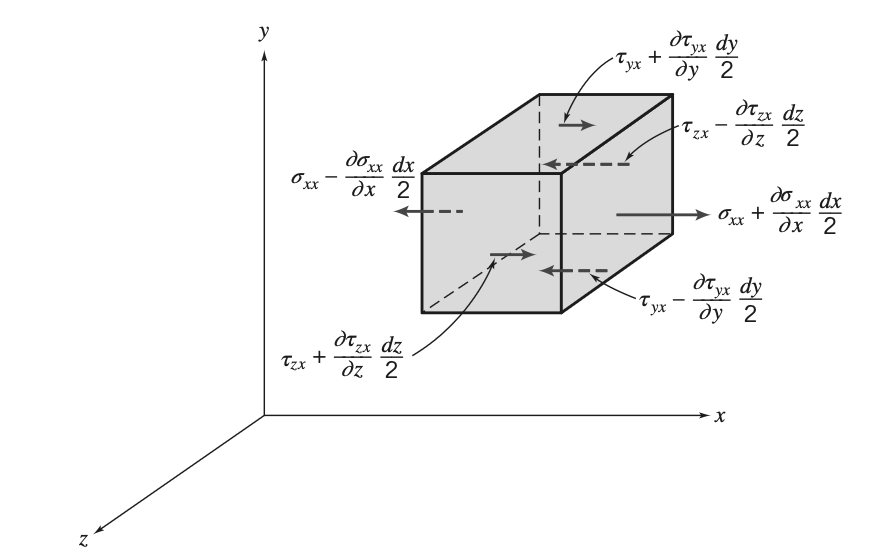
\includegraphics[width=0.8\linewidth]{./figures/f5_9.png}
  \caption{Stresses in the $x$ direction on a fluid element.}
  \label{fig:f5_9}
\end{figure}
To obtain the net surface force in the $x$ direction $\mathrm{d}F_{S_x}$ we must sum the forces in the $x$-direction. On simplifying this we obtain:
\[ 
\mathrm{d}F_{S_x} = \left( \frac{\partial \sigma_{x x}}{\partial x} + \frac{\partial \tau_{yx}}{\partial y} + \frac{\partial \tau_{zx}}{\partial z} \right) \, \mathrm{d}x \, \mathrm{d}y \, \mathrm{d}z
.\]
Assuming the gravitational force is the only body force acting on the system, then the net force in the $x$ direction $\mathrm{d}F_x$ is given by:
\[ 
\mathrm{d}F_x = \mathrm{d}F_{B_x} + \mathrm{d}F_{S_x} = \left( \rho g_x + \frac{\partial \sigma_{x x}}{\partial x} + \frac{\partial \tau_{yx}}{\partial y} + \frac{\partial \tau_{zx}}{\partial z}  \right) \, \mathrm{d}x \, \mathrm{d}y \, \mathrm{d}z
.\]
Similarly for the force in the $y$ and $z$ directions:
\begin{align*}
  \mathrm{d}F_y &= \mathrm{d}F_{B_y} + \mathrm{d}F_{S_y} = \left( \rho g_y + \frac{\partial \tau_{x y}}{\partial x} + \frac{\partial \sigma_{yy}}{\partial y} + \frac{\partial \tau_{zy}}{\partial z}  \right) \, \mathrm{d}x \, \mathrm{d}y \, \mathrm{d}z \\
  \mathrm{d}F_z &= \mathrm{d}F_{B_z} + \mathrm{d}F_{S_z} = \left( \rho g_z + \frac{\partial \tau{x z}}{\partial x} + \frac{\partial \tau_{yz}}{\partial y} + \frac{\partial \sigma_{zz}}{\partial z}  \right) \, \mathrm{d}x \, \mathrm{d}y \, \mathrm{d}z
.\end{align*}

\subsubsection{Differential Momentum Equation}
Now we have defined the force components acting on a fluid element of mass $\mathrm{d}m$. If we substitute these expressions into Newton's second law from before we obtain the differential equations of motion,
\begin{align*}
  \rho g_x + \frac{\partial \sigma_{x x}}{\partial x} + \frac{\partial \tau_{yx}}{\partial y} + \frac{\partial \tau_{zx}}{\partial z} &= \rho \left( \frac{\partial u}{\partial t} + u \frac{\partial u}{\partial x} + v \frac{\partial u}{\partial y} + w \frac{\partial u}{\partial z}  \right) \\
  \rho g_y + \frac{\partial \tau_{xy}}{\partial x} + \frac{\partial \sigma_{yy}}{\partial y} + \frac{\partial \tau_{zy}}{\partial z} &= \rho \left( \frac{\partial v}{\partial t} + u \frac{\partial v}{\partial x} + v \frac{\partial v}{\partial y} + w \frac{\partial v}{\partial z}  \right) \\
  \rho g_z + \frac{\partial \tau_{xz}}{\partial x} + \frac{\partial \tau_{yz}}{\partial y} + \frac{\partial \sigma_{zz}}{\partial z} &= \rho \left( \frac{\partial w}{\partial t} + u \frac{\partial w}{\partial x} + v \frac{\partial w}{\partial y} + w \frac{\partial w}{\partial z}  \right)
.\end{align*}
These are the differential equations of motion for any fluid satisfying the continuum assumption. 

\subsubsection{Newtonian Fluid: Navier-Stokes Equations} \label{sec:navsto}
For a Newtonian fluid the viscous stress is directly proportional to the rate of shearing strain (the angular deformation rate). The stresses may be expressed in terms of velocity gradients and fluid properties in rectangular coordinates as:
\begin{align*}
  \tau_{xy} &= \tau_{yx} = \mu \left( \frac{\partial v}{\partial x} + \frac{\partial u}{\partial y}  \right) \\
  \tau_{yz} &= \tau_{zy} = \mu \left( \frac{\partial w}{\partial y} + \frac{\partial v}{\partial z}  \right) \\
  \tau_{zx} &= \tau_{xz} = \mu \left( \frac{\partial u}{\partial z} + \frac{\partial w}{\partial x}  \right) \\
  \sigma_{x x} &= - p - \frac{2}{3} \mu \nabla \textbf{V} + 2 \mu \frac{\partial u}{\partial x}  \\
  \sigma_{yy} &= -p - \frac{2}{3} \mu \nabla  \textbf{V} + 2 \mu \frac{\partial v}{\partial y}  \\
  \sigma_{zz} &= -p - \frac{2}{3} \mu \nabla  \cdot \textbf{V} + 2 \mu \frac{\partial w}{\partial z} 
.\end{align*}
There $p$ is the local pressure. If these expressions for the stresses are introduced into the differential equations of motion we obtain:
\begin{align*}
  \rho \frac{\mathrm{D}u}{\mathrm{D}t} &= \rho g_x - \frac{\partial p}{\partial x} + \frac{\partial }{\partial x} \left( \mu \left( 2 \frac{\partial u}{\partial x} - \frac{2}{3} \nabla  \cdot \textbf{V} \right) \right) + \frac{\partial }{\partial y} \left( \mu \left( \frac{\partial u}{\partial y} + \frac{\partial v}{\partial x}  \right) \right) + \frac{\partial }{\partial z} \left( \mu \left( \frac{\partial w}{\partial x} + \frac{\partial u}{\partial z}  \right) \right) \\
  \rho \frac{\mathrm{D}v}{\mathrm{D}t} &= \rho g_y - \frac{\partial p}{\partial y} + \frac{\partial }{\partial x} \left( \mu \left( \frac{\partial u}{\partial y} + \frac{\partial v}{\partial x}  \right) \right) + \frac{\partial }{\partial y}\left( \mu \left( 2 \frac{\partial v}{\partial y} - \frac{2}{3} \nabla \cdot \textbf{V} \right) \right) + \frac{\partial }{\partial z} \left( \mu \left( \frac{\partial v}{\partial z} + \frac{\partial w}{\partial y}  \right) \right) \\
  \rho \frac{\mathrm{D}w}{\mathrm{D}t} &= \rho g_z - \frac{\partial p}{\partial z} + \frac{\partial }{\partial x} \left( \mu \left( \frac{\partial w}{\partial x} + \frac{\partial u}{\partial z}  \right) \right) + \frac{\partial }{\partial y}\left( \mu \left( \frac{\partial w}{\partial z} + \frac{\partial w}{\partial y}  \right) \right) + \frac{\partial }{\partial z} \left( \mu \left( 2 \frac{\partial w}{\partial z} - \frac{2}{3} \nabla \cdot \textbf{V} \right) \right)
.\end{align*}
These equations of motion are called the \textit{Navier-Stokes equations}. For an incompressible flow these reduce to:
\begin{align*}
  \rho \left( \frac{\partial u}{\partial t} + u \frac{\partial u}{\partial x} + v \frac{\partial u}{\partial y} + w \frac{\partial u}{\partial z}  \right) &= \rho g_x - \frac{\partial p}{\partial x} + \mu \left( \frac{\partial^2 u}{\partial x^2} + \frac{\partial^2 u}{\partial y^2} + \frac{\partial^2 u}{\partial z^2} \right) \\
  \rho \left( \frac{\partial v}{\partial t} + u \frac{\partial v}{\partial x} + v \frac{\partial v}{\partial y} + w \frac{\partial v}{\partial z}  \right) &= \rho g_y - \frac{\partial p}{\partial y} + \mu \left( \frac{\partial^2 v}{\partial x^2} + \frac{\partial^2 v}{\partial y^2} + \frac{\partial^2 v}{\partial z^2} \right) \\
  \rho \left( \frac{\partial w}{\partial t} + u \frac{\partial w}{\partial x} + v \frac{\partial w}{\partial y} + w \frac{\partial w}{\partial z}  \right) &= \rho g_z - \frac{\partial p}{\partial z} + \mu \left( \frac{\partial^2 w}{\partial x^2} + \frac{\partial^2 w}{\partial y^2} + \frac{\partial^2 w}{\partial z^2} \right)
.\end{align*}
These describe many common flows so long as the fluids are Newtonian and incompressible. 
